\chapter{Results}
\label{chapter3}

\section{Alpha Testing}

\subsection{Special Moves}
\label{SpecialMoves}

This was briefly mentioned in section \ref{TheChessPage} but now we will look into the process that went into testing the special moves that you can make in chess. Each one required new systems to be built into the back and front end in order to function correctly, which is what makes these moves so special.

We will start with promotion. This is the act of moving your pawn to the very end of the board, at which point you can choose to "promote" it to another piece (choosing from Queen, Rook, Knight and Bishop). In this case, the new square should instead show the piece selected by the user. The user can select this piece through a menu that we have designed, which features four icons representing the four pieces. Using the mouse or the touch screen, a user can select the piece and the data is sent by the client to the server, to inform it of the decision. The server sends back a generic message that will update the board as expected.

Moving onto the second case, we have en passant. In this case, the piece that we capture (take) is not on the same space that our piece moves to. Before we changed the code, the piece would be removed from the board on the back end but it would look like it is still there on the front end. To fix this, the server sends an additional message after the "play" message to clear the space of the pawn we have just captured.

Finally we have castling, which is the most complex of them all. When the king attempts to castle, we first need to work out the rank and file (row and column) of the rook that the king is castling with and the end position for it. We send the normal "play" message for the king and then a second "play" message for the rook. This had an unforeseen consequence of toggling the turn prompt twice on the front end so it would look like the user could move again after castling. This however is only a visual glitch and the server continues to hold the correct turn value on the back end. The reason for this is because the front end toggles the turn to switch between white and black when a user makes their move, which is usually what we want. To resolve this, we can add a flag, called "contribute turn", that alerts the front end whether this move should toggle the turn prompt. This value will default to true because this is the behaviour we would expect in most cases, however when we send the second play for the rook, we will set this flag to false.

\subsection{Responsive Design}

A minor problem for the responsive design arose when testing on an Apple iPhone, using the Safari browser. The css for the body element was set to 100vh\footnote{vw/vh represent 1\% of the viewport's width and height respectively, therefore 100vh should, in theory, equate to 100\% of the viewport.}, as this works fine on desktop computers, however for iPhone, this value is not very intuitive. After testing, it appeared that the graphical user interface was included in the view port (such as the search bar), so certain elements would be hidden behind Safari's interface. This article \cite{100vhFix}, written by Trzciński M., provided some useful code, which was implemented in our own codebase. This addition was able to fix the issue and allowed all the elements to display correctly on the page and adapt when the GUI (graphical user interface) was minimised.

An additional problem, which is difficult to replicate (and therefore difficult to fix) occurred when using the developer tools during a chess game. When opening the developer tools on the side, the content of the page would half in size and it caused problems when mapping mouse clicks to a square on the board. However, by trying to force it to happen and having no success is a good sign because it means its a rare bug, but it would be better to know the root cause and deal with it accordingly but it is beyond the scope of this project.

\subsection{The End Game}

A benefit of using the python-chess module is the ability to provide the board class with a fen string to initialise the pieces on the board; this was especially useful for quickly testing the stalemate condition. The fen we are using to test/demonstrate stalemate is \emph{5b2/8/8/8/8/n7/PP6/K7 b}\footnote{This is not a full fen string but the module provides defaults for the remaining values, which is fine, because we only care about the positions and turn for this example}. As we can see in figure \ref{EndGameExamples}, we move the bishop from f8 to g7 and as we expect, a stalemate is reached. The text at the top of the page also reflects this.

The other end game is Checkmate and this can be attained quickly from the initial position. This is achieved by a set of moves called the "Fool's Mate", which has been recognised since the 17th century \cite{FoolsMateBook}. There are minor variations in the way this Checkmate can be achieved, in figure \ref{EndGameExamples}, the moves are as follows:
\begin{enumerate}
    \item f4, e5
    \item g4, Qh4\#
\end{enumerate}
Similar to the stalemate, by making these moves, we can reach and endgame and the text at the top will indicate that the condition by which the game has ended is indeed "Checkmate". This used to be the only thing that happened at the end of the game, however an extra visual has been added as a result of user feedback, more detail will be provided in section \ref{VisualsFeedback}.

\begin{figure}[h]
    \begin{center}
        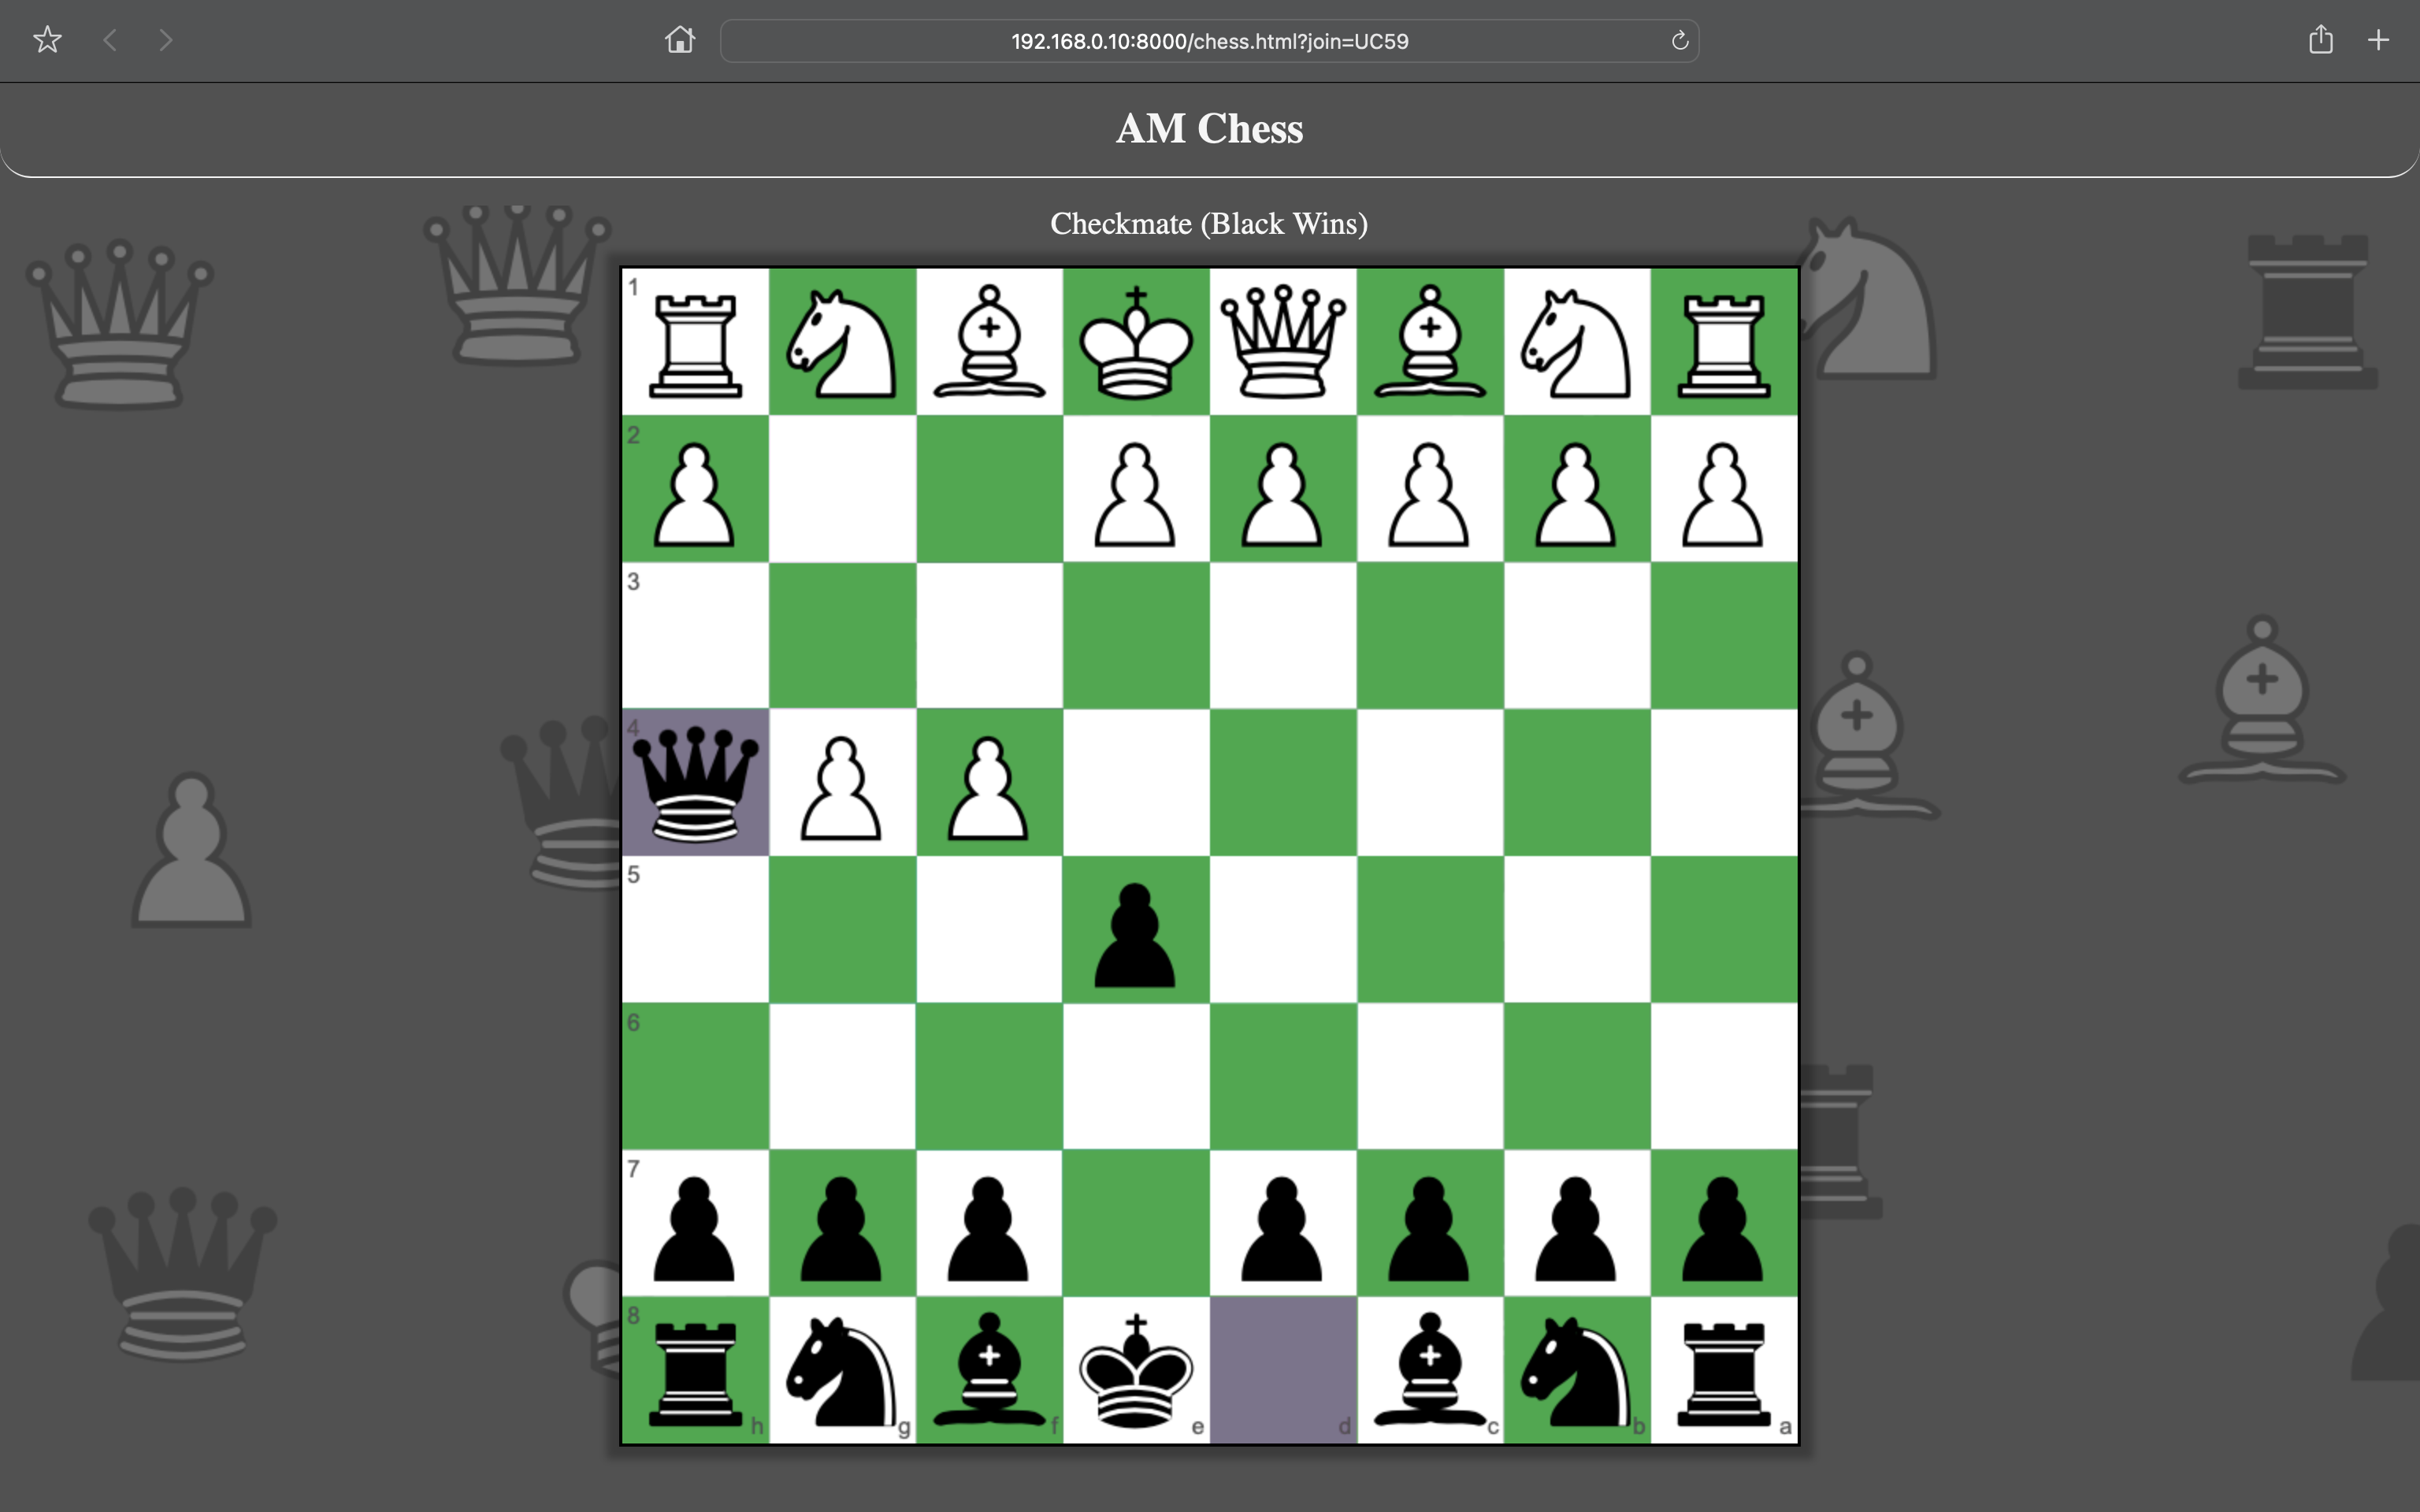
\includegraphics[width=0.45\textwidth]{FoolsMate}
        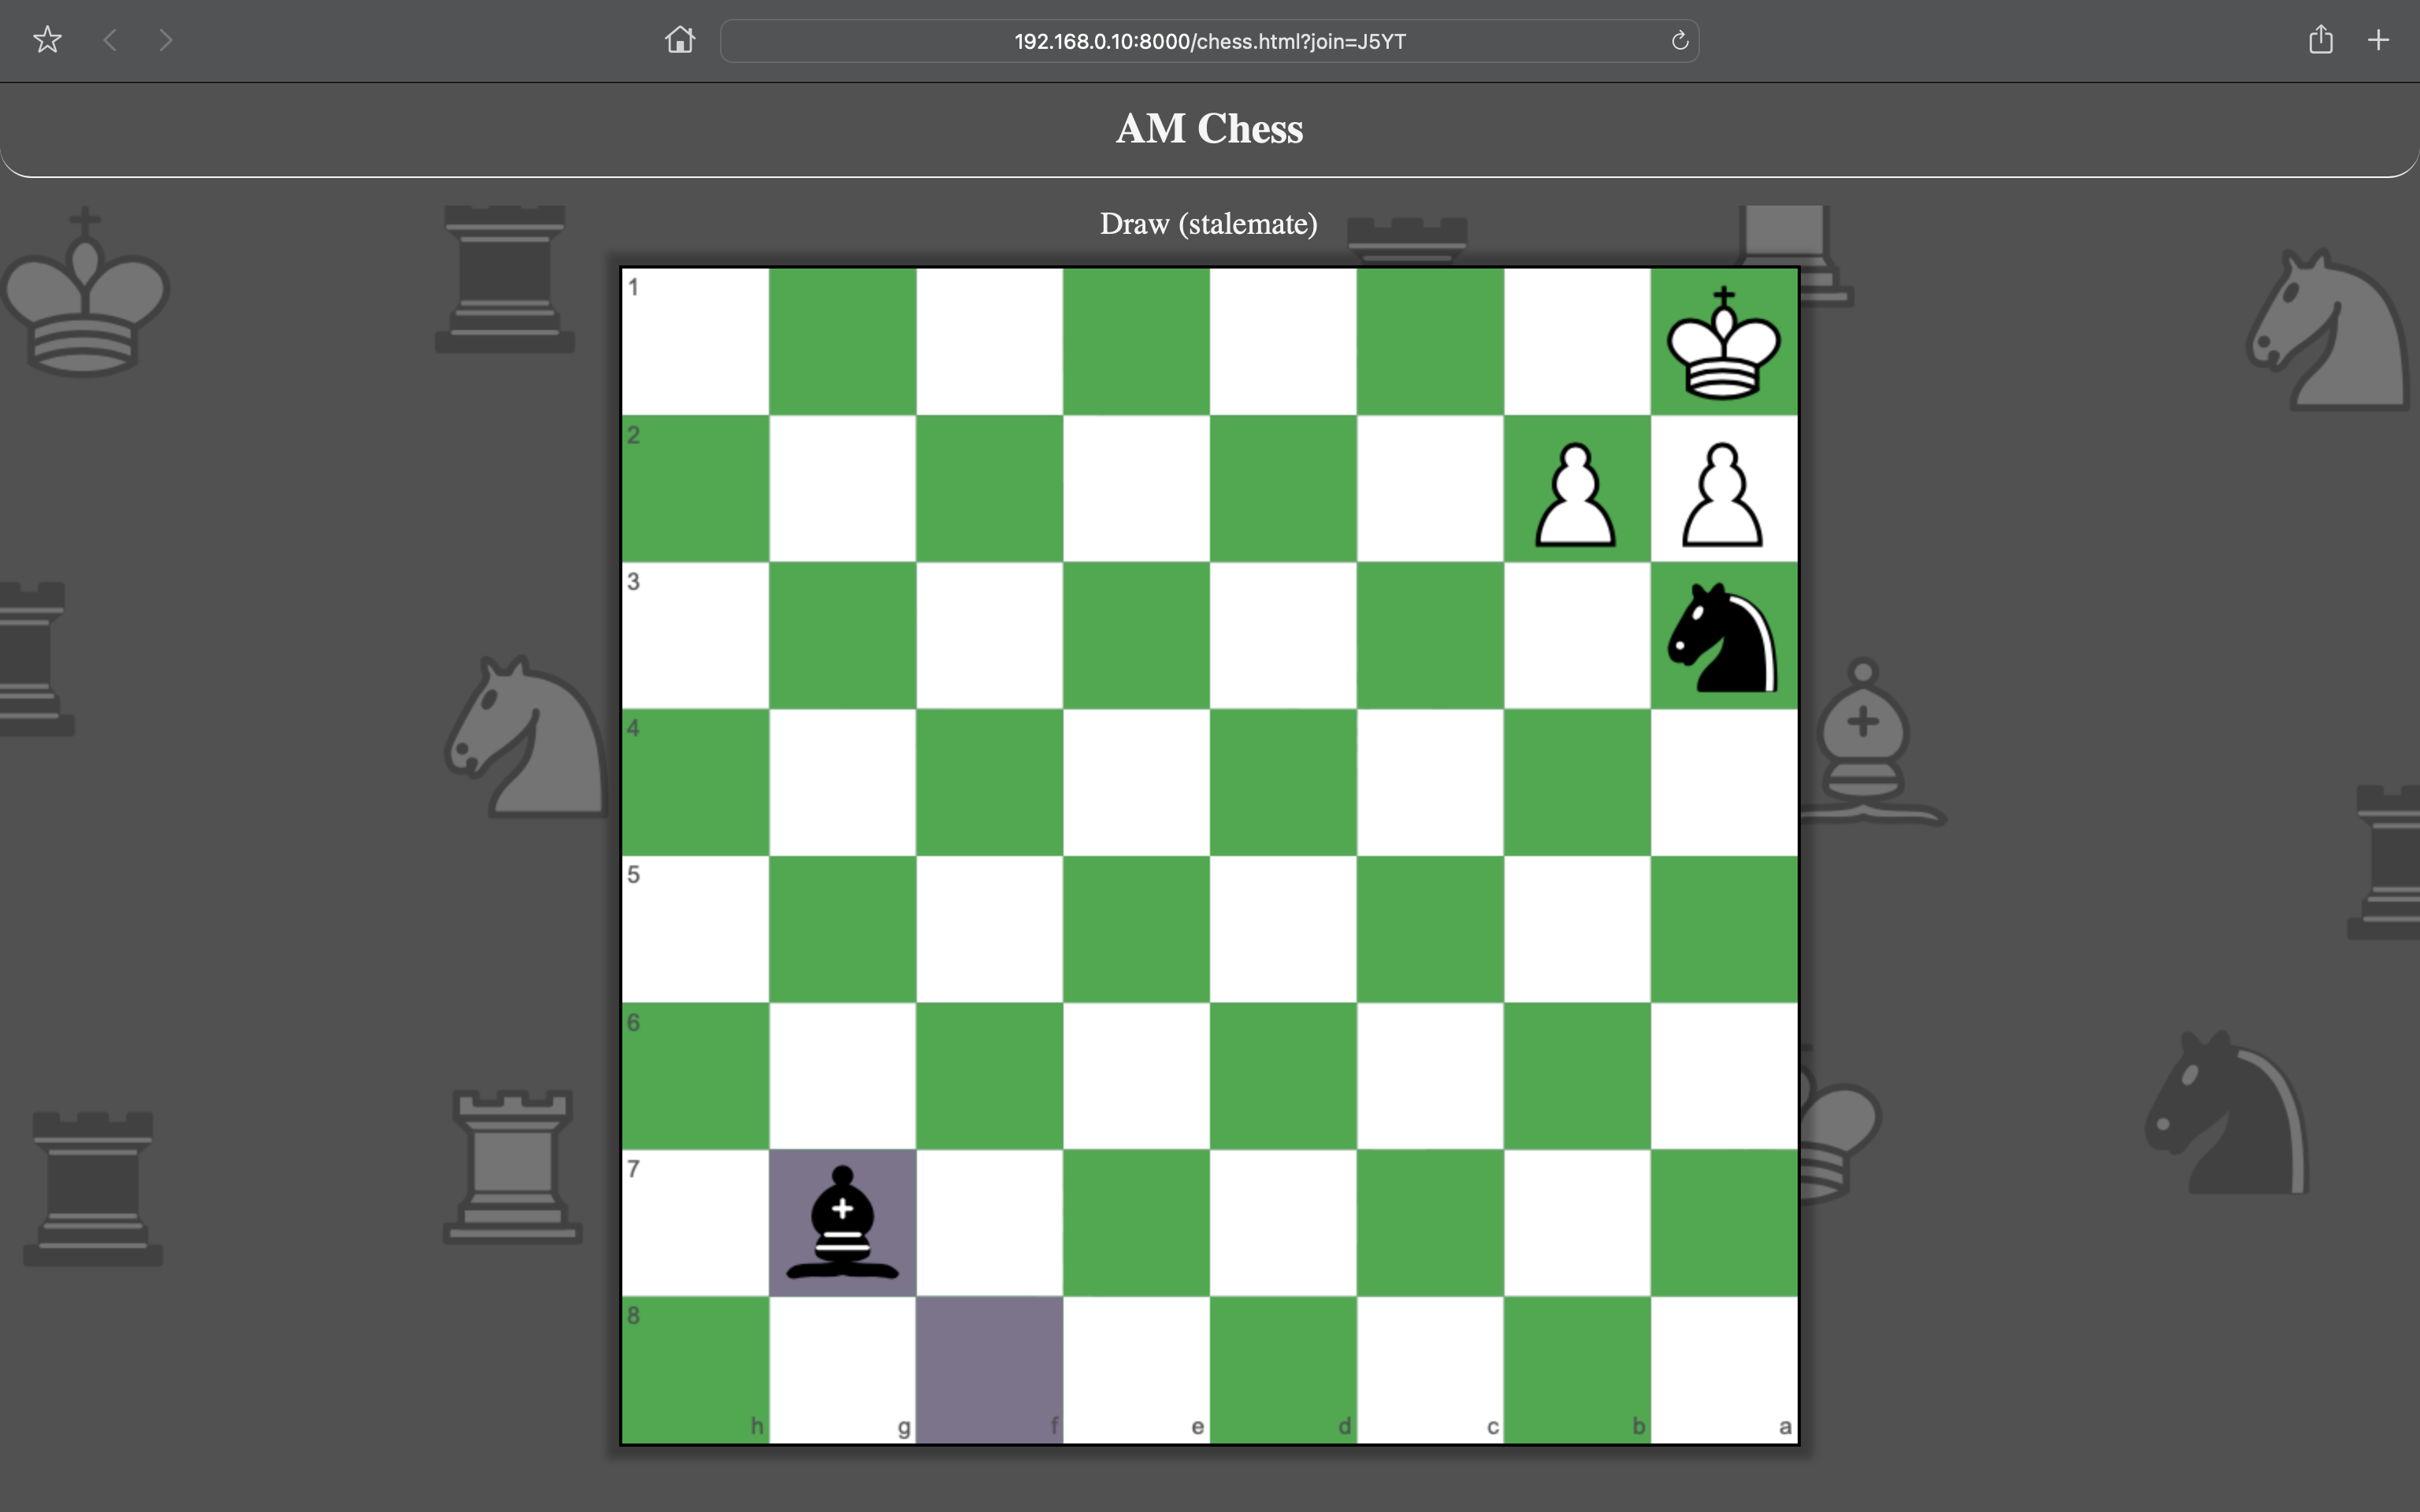
\includegraphics[width=0.45\textwidth]{Stalemate}
        \caption{Two end states, Checkmate via "Fool's Mate" in 2 moves on the left and a Stalemate on the right}
        \label{EndGameExamples}
    \end{center}
\end{figure}

\subsection{No Game}

When testing this app, we have to start two servers, the http server to send web pages and supporting files, and the websocket server to handle requests and game logic. However, the fact that the websocket server might not be running was never considered. This led to a confusing series of events, when staring at a blank page and wondering "why it was working the day before but not today?". As one could guess, it's because the websocket server was not running. This revealed a hole in our codebase and it needed to be plugged. Before we dive into the solution, it's important to know that an event is triggered by a websocket when it closes; when a socket tries to connect to a server and fails, this is included as a close. Therefore when the program first starts, if it detects a close event, it will alert the user that the server is not operating and will set a timeout that will send the user back to the homepage.

\begin{figure}[h]
    \begin{center}
        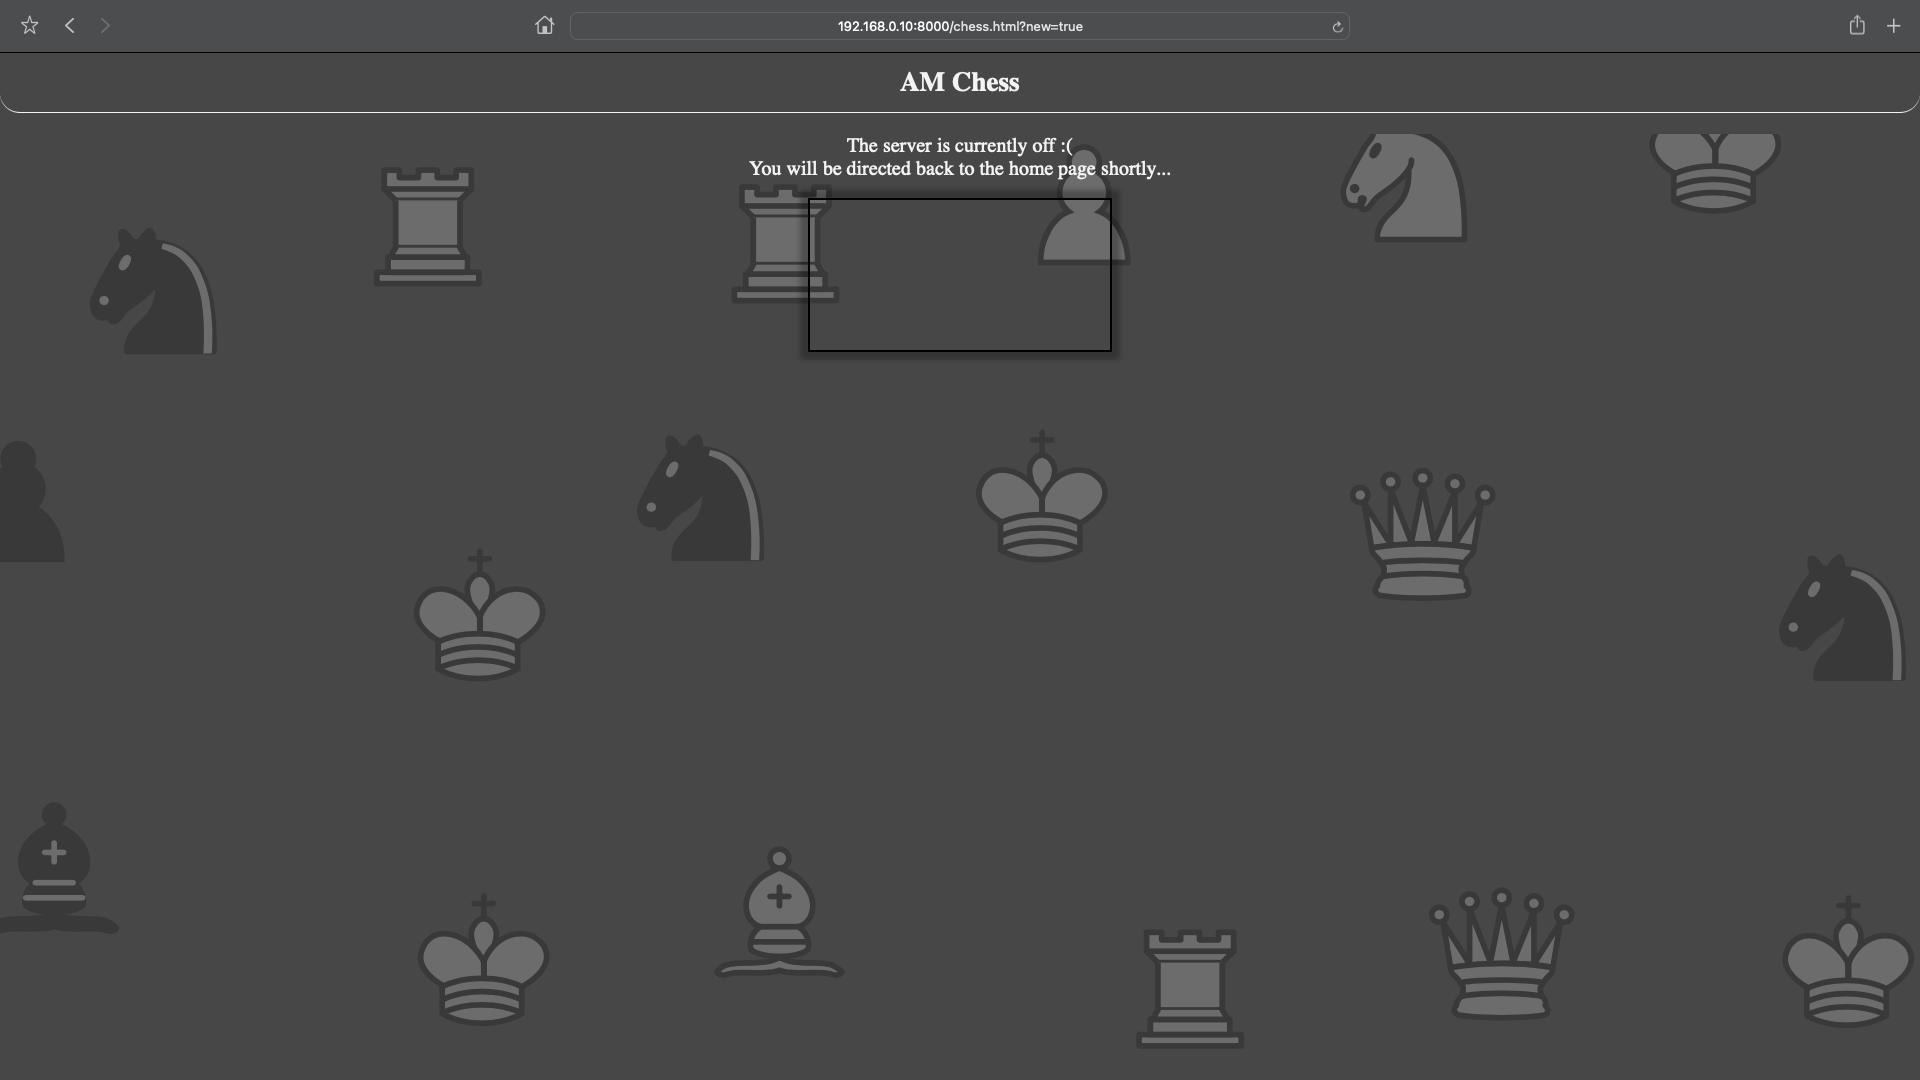
\includegraphics[width=0.5\textwidth]{NoGameExample}
        \caption{The chess page when the server has crashed or switched off}
    \end{center}
\end{figure}

Another way in which a user could be redirected to the homepage is by manually typing the url in the search bar. In general the chess.html page takes one of two query parameters:

\begin{enumerate}
    \item new=true
    \item join={JOIN\_KEY}
\end{enumerate}

Where we replace JOIN\_KEY, with a valid 4 character code. However if a user intentionally enters a url that does not follow this structure, the browser will alert them and send them back to the home page. By testing all these edge cases we are able to evaluate the current responses, which in this case is an empty page, and make a decision as to what should happen instead. This refinements are what will lead to a smoother experience for the user.

\subsection{Connection Issues}

As an aside, I had an interesting experience while the app was in early stages of testing, when I was traveling by train and would occasionally lose my connection to the internet while going through tunnels. My app was able to survive this disturbance and using the reconnect button as described in section \ref{Websockets}, I was able to continue testing the app as normal. Even though it was developed for other circumstances, it was nice to see it also supporting other situations as well.

\section{User Testing and Feedback}
\label{UserTestingAndFeedback}

User feedback was collected through google forms and the automatically generated spreadsheet can be accessed via the following link:
\begin{center}
    \url{https://docs.google.com/spreadsheets/d/1DjMKbAfgBAj0ksE6rK4WPJBflKK6LeDs_MvxAArTZa0/edit?usp=sharing}
\end{center}

There is only so much testing we can do as developers before we need to outsource our tests to other, consenting users. A side effect of being involved in the development is that we are unable to simulate the experience of a new user. We know exactly how the app functions and can navigate with ease, but can we say the same for people visiting our app for the first time? We will discuss this in the following sections.

The first part of the feedback form helps us gauge the diversity of our sample, by asking questions about the user's background with chess. By looking at figure \ref{StatDiversity} we can see that we have a mix of experienced chess players and those who are new to the scene. This is beneficial to us because different people want different things, and all of this feedback can be processed and implemented to create a program that is enjoyed by everyone. For example, the experienced players want features that they are used to, like the ability to draw on the board in order to plan their next move. Meanwhile, new users want features that will help them play the game, by giving instructions on the rules and even possibly hints on what move they should make. 

\begin{figure}
    \begin{center}
        \fbox{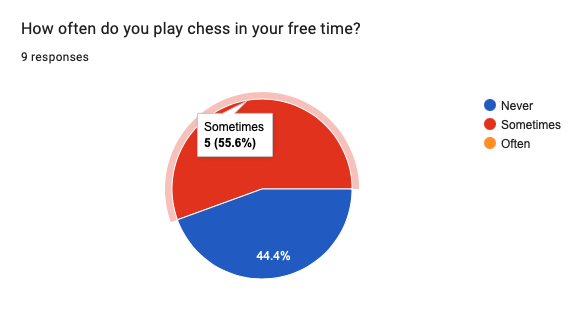
\includegraphics[width=0.5\textwidth]{StatPlayFrequency}} \\
        \vspace{1cm}
        \fbox{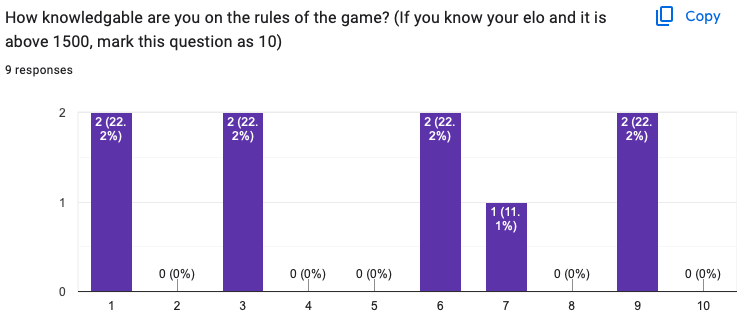
\includegraphics[width=0.5\textwidth]{StatKnowledge}}
        \caption{A pie chart depicting the frequency of how often users play chess and a bar char showing how they would rate their knowledge on the game.}
        \label{StatDiversity}
    \end{center}
\end{figure}

\subsection{Functionality}

The most important statistic to consider though, is the percentage of players who were able to start and finish a game of chess... Which was 100\% of the participants! Despite the range of people who tested our app, every single person was able to play at least one game of chess until the end, which was the main objective of this project! Additionally, the user's were able to easily navigate through the app and the user interface made sense. This is backed up by the 88.9\% of testers that said they were never in a situation where they didn't know how to progress. While the features that were implemented were easy to use, there were a few features that users would have liked to see, so we will discuss those now and what we have done about it.

\subsubsection{Where did you move?}

A common question that was said during the tests involved asking the opponent what piece they had just moved. Depending on who you play against, they may not be so willing to answer in order to gain an slight advantage. To eliminate this problem, we can learn from the feedback and implement a means of visualising the most recent move that was made. The feature has subtly made an appearance already in figure \ref{EndGameExamples}, through the form of translucent pink squares. These are drawn where the piece has moved from as well as where it has moved to. For reference, this would be the queen from d8 to h4 on the left and bishop from f8 to g7 on the right.

\subsubsection{Responsiveness}

As an online application, responsiveness is an important factor to consider when thinking about the user experience. When deciding where the location for the websocket server, Europe was chosen as that is the closest location to where all users will be testing. The responsiveness condition was clearly met when looking at the user feedback where 88.9\% of users rated the responsiveness as 5/5. The one tester who rated 4/5, also commented in the optional box that the responsiveness was "perfect", so there may have been some misunderstanding when they gave their rating. This test only considers participants in Europe, unfortunately there was no one reliable to test with outside of this area, so we can only say for certain that it is responsive in Europe and nothing concrete can be said for continents outside of this area.

\subsubsection{Game Keys}

It was surprising to see that no one had mentioned having issues with the game keys. It wasn't considered until testing had commenced but the characters 0 and O are very similar and this could be confusing to those who are trying to join a game. Even though no one had commented on this as an issue, it would be wise to remove one of these characters to avoid the potential for confusion in the future.

\subsection{Visuals}
\label{VisualsFeedback}

A goal of the project was not only for it to be functional but also visually pleasing; some of the changes may already be noticeable from the figures earlier in this chapter. After taking some feedback into consideration, the website now looks more polished and cohesive. The colour palette has changed to monochrome and this pairs well with the black and white pieces. Additionally, the neutral colours allow for important text like hints to stand out; this also has the same effect for the board. Additional effects, such as a border and shadow, were also implemented for the board and this gives it more depth and makes it stand out even more. After all, the board is the most important part of this app, so it should have the main focus. The board not maintains more of its colour too because the highlighting for available moves is now translucent, which means you can still see a part of the original colour underneath.

The background of the website has also been updated and it reuses assets we have already implemented for the game. Upon entering the website, the program pseudo-randomly draws chess pieces to the background. From previous experience, when "programmer art" is left to  complete random, it is never usually pleasing to look at. Hence why the positioning is only random, to a degree. The way the position algorithm works, is by diving the background into cells and only considering every other cell. We then generate a random value to offset the position, this is capped to ensure that no two pieces overlap. Finally the background has its opacity lowered so it is not confused with the foreground elements. This change was suggested by one of the testers on the questionnaire and it definitely improves the overall feel and quality of the app. The effects can be seen in figure \ref{welcomePageUpdated}.

\begin{figure}
    \begin{center}
        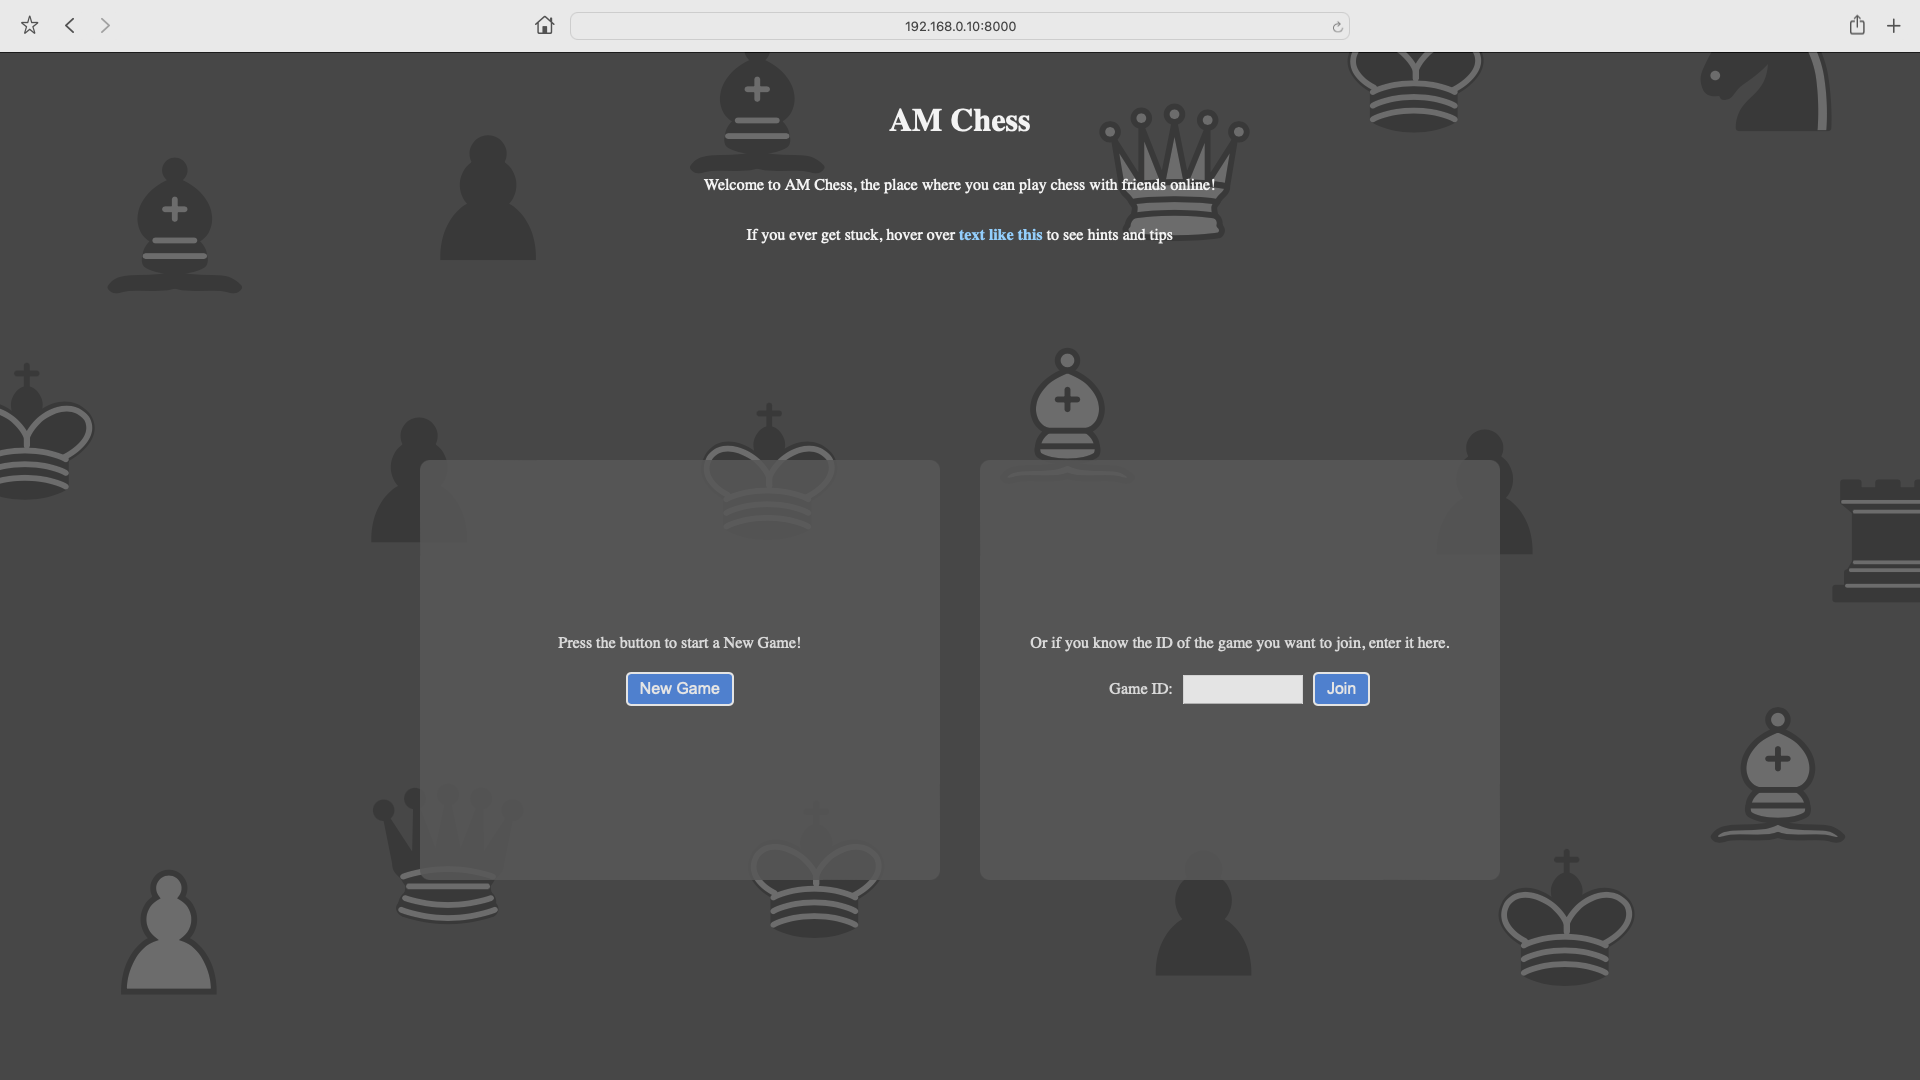
\includegraphics[width=0.75\textwidth]{welcomePageUpdated}
        \caption{The welcome page with updated visuals, welcoming text and important information relating on how to interact with the hint system}
        \label{welcomePageUpdated}
    \end{center}
\end{figure}

An interesting visual feature was hinted to earlier and it's something that occurs if someone \emph{wins}, and only if someone wins. This feature is a confetti canon that shoots multicoloured confetti around the screen. This was developed using a basic, custom made particle system. Being completely separate from everything else, this code was developed in its own file and is imported in the "game.js" file and is executed during the "win" function. This was added to provide some recognition to a user's win because multiple people commented on the anti-climatic feeling of completing a game. A figure will not be provided for this feature because a still picture would not do it justice. A demonstration of the fanfare can be seen in the demo video, which can be found in section \ref{Conclusion}.

\subsection{Audio}

Despite it appearing in all 3 examples in section \ref{ExistingSolutions}, sound was not considered for this project. This was a mistake because sound plays a big role in immersion as well as indicating that a move has been made. As mentioned in the previous section, there is now an added visual for the last move that has been made. This is definitely a step in the right direction but after first hand experience and looking at the user feedback, it is clear that an auditory que would be beneficial. Unlike the text, that could go unnoticed, a sound is much more likely to alert a user that it is their turn. From observation, a lot of time was spent for both people waiting for each other to make a move, hopefully adding sound would make this less of an issue.

\subsection{Inexperienced Players}

Finally we will look at the feedback given by users who are new to chess. One of the testers said that they didn't know what check was and why they were not allowed to move certain pieces during this time. After hearing this feedback, we can include elements with certain traits that can offer advice. This is implemented with bold text in a unique colour, to indicate that it is interact-able. A user can either hover over it with their mouse on a computer or press it on their touchscreen device. This will cause the corresponding text to explain the current situation. So in this example, when a user is in check, if they hover over the "(In check)" text, they will see a prompt that reads: "Check means that a piece is attacking the king and he needs to get out of danger". A user is made aware of this functionality from the welcome page, where it explains explicitly how to view hints and tips. There is even an example on the page to reinforce the learning. After accessing the hint, it remains on the screen for 5 seconds. It used to appear for less time because there isn't a lot to read. However, from previous experience, this is a naïve thought to have because it is quicker to read text when you've written it yourself and already know what it says. Therefore, it will stay on the page for longer. Even though some users may be able to read it with lots of time spare, it is better to implement it this way so that it is accessible for more users.

Due to both the welcome page and chess page using hints, we have written the functionality in a new file that is included in both web pages. The file contains an entry function that accepts a "hint anchor" element - the text we hover over, and a "hint text" element - the text that includes the hint. The function then assigns the necessary event listeners to the anchor, including mouseenter and mousemove. To add some life to the prompt, if a person uses their mouse, the prompt will follow the mouse (so long as the mouse continues to hover over the anchor text). The ability of encapsulating the code to make something "hover-able" (to have an effect when hovered over), means it can be used multiple times but only written once, which aligns with the DRY (don't repeat yourself) principles. It means we can also assign it to elements easily during runtime. The best example of this is the turn text. This element is not usually hover-able, but if a user attempts to move when it is not their turn it becomes red and hover-able. This was also the result of a change from user feedback, where a user did not like receiving a browser error message for an in game error. So now when a user hovers over the (red) turn text, it will emphasise that it is not their turn. The text will eventually go back to normal after sometime, meaning it is also no longer hover-able anymore. This is managed by a second function that does the opposite of the first function and simply removes the event listeners and the class attributes that give it the hover-able look (e.g. bold font weight).

\begin{figure}
    \begin{center}
        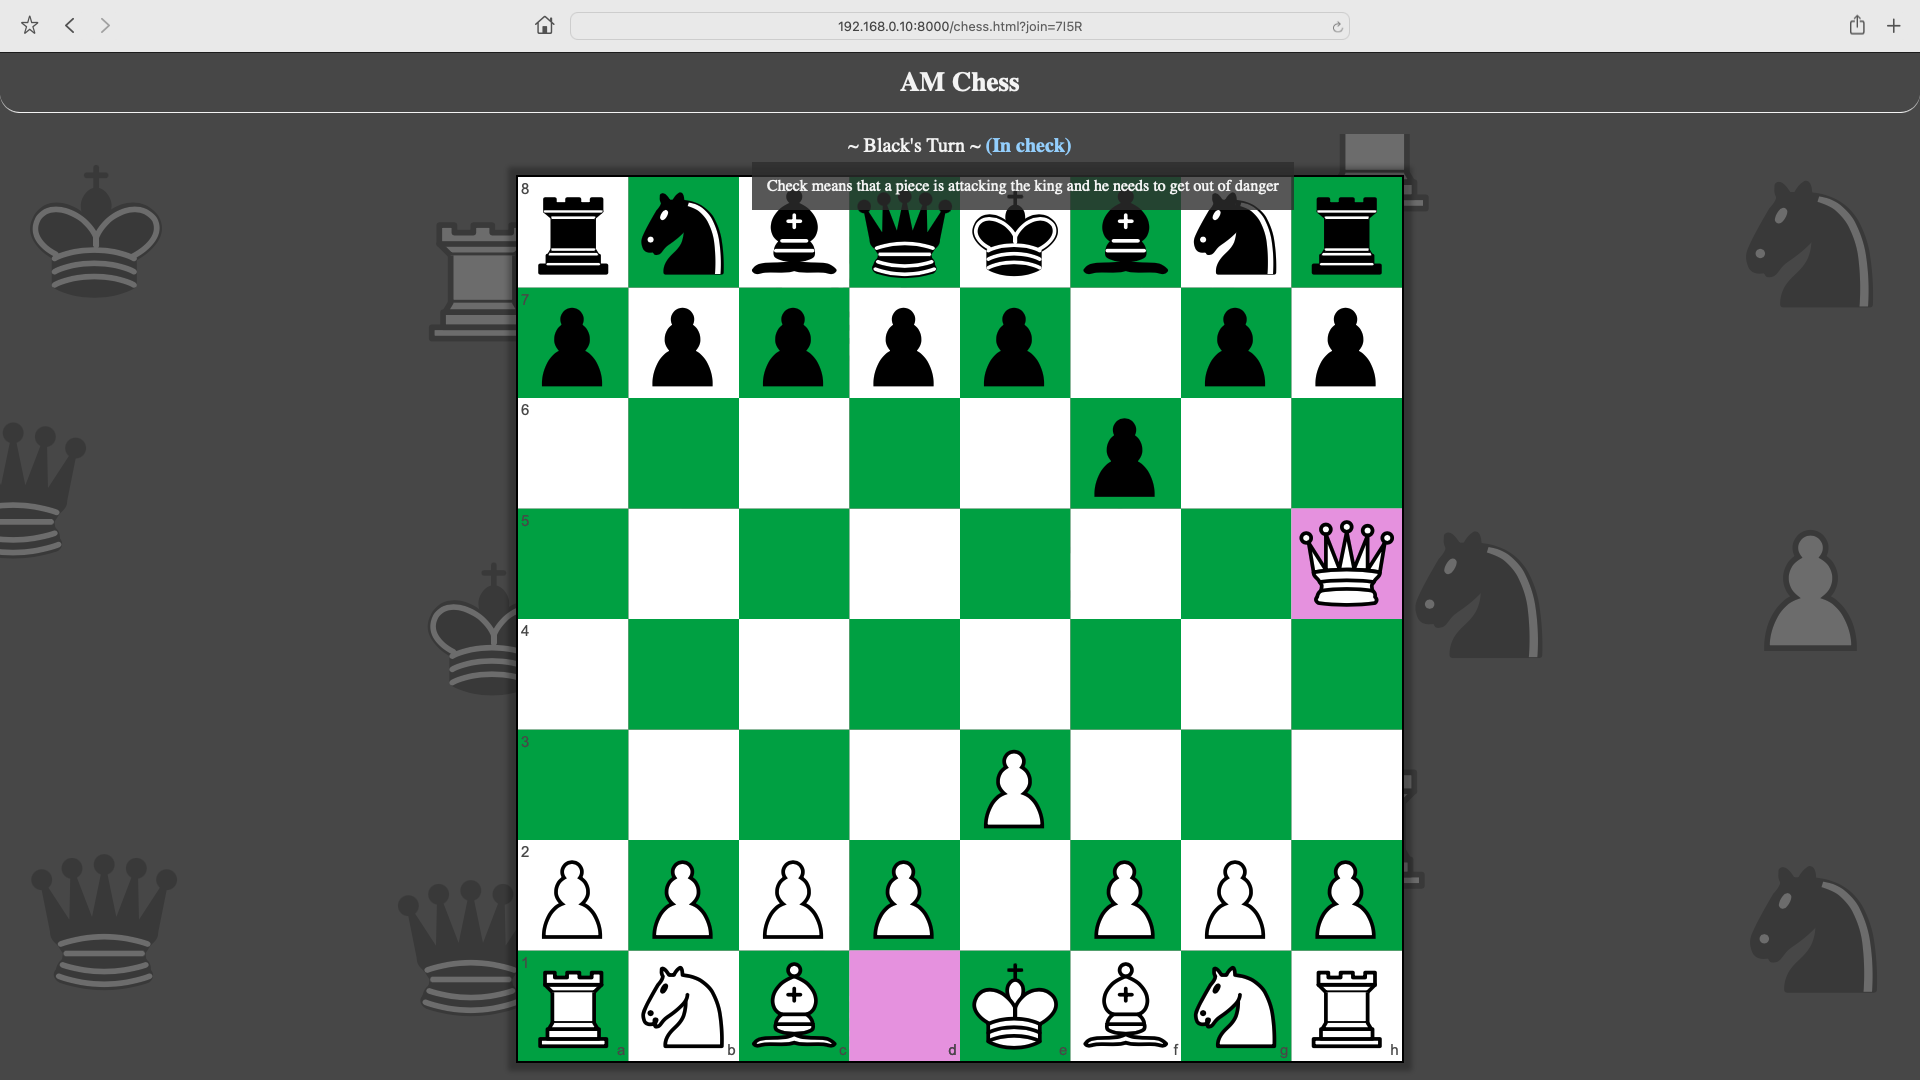
\includegraphics[width=0.75\textwidth]{hoverExample}
        \caption{Demonstration of using the hover hint feature}
        \label{hoverExample}
    \end{center}
\end{figure}
